\documentclass[conference]{IEEEtran}
\IEEEoverridecommandlockouts
% The preceding line is only needed to identify funding in the first footnote. If that is unneeded, please comment it out.
\usepackage{cite}
\usepackage{amsmath,amssymb,amsfonts}
\usepackage{algorithmic}
\usepackage{graphicx}
\usepackage{textcomp}
% \usepackage[utf8]{vietnam}
\usepackage{xcolor}
\usepackage{booktabs}
\usepackage{float}
\usepackage{tabularx}
\usepackage[numbers, square]{natbib}
\usepackage{hyperref}
\def\BibTeX{{\rm B\kern-.05em{\sc i\kern-.025em b}\kern-.08em
    T\kern-.1667em\lower.7ex\hbox{E}\kern-.125emX}}
\begin{document}

\graphicspath{{Image/}}

% \title{Chatbot with an Integrated Question Suggestion System for E-commerce Platforms}
\title{Conversational Product Navigation for E-commerce via Knowledge-Based Multi-Agent Chatbots
}

\author{\IEEEauthorblockN{Tien-Thanh Pham}
\IEEEauthorblockA{\textit{School of Information and Communications Technology} \\
\textit{Hanoi University of
Science and Technology}\\
Hanoi, Vietnam \\
tienthanhtk11@icloud.com}
\and
\IEEEauthorblockN{Tuan-Dat Trinh\IEEEauthorrefmark{1}}
\IEEEauthorblockA{\textit{School of Information and Communications Technology} \\
\textit{Hanoi University of
Science and Technology}\\
Hanoi, Vietnam \\
dat.trinhtuan@hust.edu.vn}
}


\IEEEoverridecommandlockouts
\makeatletter
\def\@IEEEpubidpullup{2\baselineskip} % Số càng lớn thì càng đẩy xuống thấp
\makeatother

\IEEEpubid{
\begin{minipage}{\textwidth}
\textsuperscript{\textsection}The two authors contributed equally to this work \\
\IEEEauthorrefmark{1}Corresponding author
\end{minipage}
}


\maketitle
% 
\begin{abstract}
\noindent Chatbots have become essential tools on e-commerce platforms, enabling automated customer consultation and support. However, most existing chatbots remain passive, merely responding to user-initiated queries without aligning with business objectives. This paper proposes a comprehensive chatbot architecture that integrates a smart question suggestion system to proactively guide conversations toward predefined business goals while maintaining natural and user-relevant interactions. The architecture combines a product knowledge graph, which links products through shared attributes, with a multi-agent system powered by large language models (LLMs) to generate goal-oriented question suggestions. The system’s effectiveness is evaluated using a simulated user environment, demonstrating its ability to maintain engaging dialogues and steer users toward target products. The proposed chatbot thus balances user satisfaction with strategic business outcomes.



% Chatbot đang trở thành một công cụ không thể thiếu trên các nền tảng thương mại điện tử, giúp tự động hóa việc tư vấn và hỗ trợ khách hàng. Tuy nhiên, phần lớn các chatbot hiện tại hoạt động một cách thụ động, chỉ trả lời các câu hỏi do người dùng khởi tạo và chưa tối ưu hóa cho mục tiêu kinh doanh. Bài báo này đề xuất một kiến trúc chatbot toàn diện, tích hợp hệ thống gợi ý câu hỏi thông minh nhằm chủ động điều hướng cuộc trò chuyện theo các mục tiêu kinh doanh đã định trước, đồng thời vẫn duy trì sự tương tác tự nhiên và phù hợp với mối quan tâm của người dùng. Kiến trúc bao gồm một đồ thị tri thức sản phẩm (Product Knowledge Graph) để liên kết các sản phẩm dựa trên thuộc tính chung và một hệ thống đa tác tử (Multi-Agent System) sử dụng các mô hình ngôn ngữ lớn (LLM) để tạo ra các gợi ý câu hỏi. Hiệu quả của hệ thống được đánh giá thông qua một môi trường mô phỏng hành vi người dùng, cho thấy khả năng duy trì sự tương tác tự nhiên với người dùng và khả năng dẫn dắt cuộc hội thoại đến các sản phẩm mục tiêu do doanh nghiệp xác định trước. Chatbot do vậy vừa đáp ứng nhu cầu của người dùng và vừa giúp doanh nghiệp thực hiện mục tiêu kinh doanh.
\end{abstract}

\begin{IEEEkeywords}
chatbot, LLM, question suggestion, multi-agent
\end{IEEEkeywords}

\section{Introduction}
The rapid advancement of artificial intelligence (AI), particularly large language models (LLMs), has revolutionized human-computer interaction. In the e-commerce sector, chatbots have quickly become a common communication tool, enabling businesses to automate customer support, provide product information, and offer round-the-clock assistance. Modern chatbots possess semantic understanding and can respond in a natural manner, reducing users' effort in information retrieval and significantly enhancing the shopping experience.


% Sự phát triển mạnh mẽ của Trí tuệ Nhân tạo (AI), đặc biệt là các Mô hình Ngôn ngữ Lớn (LLMs), đã tạo ra một cuộc cách mạng trong lĩnh vực tương tác người-máy. Trong ngành thương mại điện tử, chatbot đã nhanh chóng trở thành một phương tiện giao tiếp phổ biến, giúp doanh nghiệp tự động hóa việc trả lời các thắc mắc của khách hàng, cung cấp thông tin sản phẩm và hỗ trợ 24/7. Các chatbot hiện đại có khả năng hiểu ngữ nghĩa và phản hồi một cách tự nhiên, giúp giảm thời gian người dùng phải tự tìm kiếm thông tin và nâng cao trải nghiệm mua sắm.


However, most existing chatbots remain limited to a reactive role. They perform well when users clearly know what they are looking for and ask direct questions. Yet, in the role of a proactive sales assistant, these systems fall short. They often lack the ability to guide, suggest, or redirect user attention toward strategic products, promotional items, or newly launched offerings that businesses aim to promote. This limitation presents a dual challenge: how to simultaneously satisfy users' information-seeking needs (user-oriented) while achieving specific business objectives (business-oriented).
% This limitation presents a dual challenge: meeting users’ information-seeking needs while simultaneously advancing business objectives.
% Tuy nhiên, vai trò của phần lớn các chatbot hiện nay vẫn còn bị giới hạn ở việc phản ứng thụ động. Chúng hoạt động hiệu quả khi người dùng biết rõ mình muốn gì và đặt câu hỏi trực tiếp. Nhưng trong vai trò của một nhân viên bán hàng chủ động, các chatbot này lại tỏ ra yếu kém. Chúng thường không có khả năng dẫn dắt, gợi mở và điều hướng sự chú ý của người dùng đến các sản phẩm chiến lược, các mặt hàng đang khuyến mãi, hay những sản phẩm mới mà doanh nghiệp muốn quảng bá. Thực trạng này tạo ra một thách thức kép: làm thế nào để vừa thỏa mãn nhu cầu tìm kiếm thông tin của người dùng (\textit{hướng người dùng - user-oriented}) vừa đạt được các mục tiêu kinh doanh cụ thể (\textit{hướng doanh nghiệp - business-oriented}).


To address these challenges, question suggestion systems represent a promising research direction. An effective system should not only generate contextually relevant questions that save users time, but also subtly guide the conversation. Achieving this requires a delicate balance between maintaining user engagement by proposing topics of potential interest and strategically steering the dialogue toward target products.

% Để giải quyết các thách thức này, các hệ thống gợi ý câu hỏi tiếp theo (next question suggestion) là một hướng nghiên cứu đầy hứa hẹn. Một hệ thống gợi ý hiệu quả không chỉ đưa ra các câu hỏi liên quan đến ngữ cảnh hội thoại, giúp người dùng tiết kiệm thời gian, mà còn phải có khả năng điều hướng cuộc trò chuyện một cách tinh tế. Việc điều hướng này đòi hỏi một sự cân bằng giữa việc duy trì sự quan tâm của người dùng bằng cách đề xuất các chủ đề họ có thể thích, và việc "lái" cuộc hội thoại đến các sản phẩm mục tiêu.


This paper proposes a comprehensive architecture for building a goal-oriented chatbot with integrated question suggestion capabilities for e-commerce platforms. The key contributions are threefold. (i) First, we construct a product knowledge graph that connects items through shared attributes, enabling logical pathways to guide conversations. (ii) Second, to support small and medium-sized enterprises that lack training data on user interaction histories, we develop a multi-agent system powered by large language models (LLMs) to both answer user queries and generate strategic question suggestions that naturally lead users toward target products. (iii) Third, to enable objective and repeatable evaluation without relying on costly user studies or potentially biased feedback from non-authentic users, we introduce an LLM-based user simulation environment.


% Bài báo này đề xuất một kiến trúc toàn diện để xây dựng một chatbot tích hợp hệ thống gợi ý câu hỏi định hướng mục tiêu cho các nền tảng thương mại điện tử với 3 đóng góp chính sau đây. (i) Chúng tôi trước tiên xây dựng một đồ thị tri thức để kết nối các sản phẩm dựa trên các thuộc tính chung, tạo ra những "con đường" logic để dẫn dắt hội thoại. (ii) Đễ hỗ trợ các doanh nghiệp vừa và nhỏ vốn không có dữ liệu huấn luyện về lịch sử tương tác của người dùng, chúng tôi sử dụng  sử dụng mô hình đa tác tử dựa trên LLM để xây dựng chatbot trả lời các câu hỏi của người dùng và một hệ gợi ý câu hỏi điều hướng người dùng đến sản phẩm đích một cách tự nhiên và hiệu quả. (iii) Để đánh giá hiệu quả, trừ khi hoạt động trong thực tiễn, dù có bố trí con người mô phỏng người dùng thật cũng sẽ không khách quan, dễ bị định kiến. Để tránh sự định kiến của con người này mà không cần cho triển khai chatbot trong một hệ thống thương mại điện tử thật, chúng tôi xây dựng một môi trường mô phỏng hành vi người dùng thực tế dựa trên LLM để lượng giá hiệu quả của hệ thống.


The remainder of the paper is organized as follows. Section~\ref{sec:related_work} reviews related work. Section~\ref{sec:knowledge_graph} presents the construction of the product knowledge graph. Section~\ref{sec:multi_agent_architecture} introduces the multi-agent system and its core components. Section~\ref{sec:user_simulation} describes the simulation setup for modeling user behavior. Section~\ref{sec:evaluation} details the experimental setup and results. Finally, Section~\ref{sec:conclusion} concludes the paper and discusses future directions.


\section{Related Work}
\label{sec:related_work}

We review prior work across three key areas: e-commerce chatbots, goal-oriented and persuasive recommendation systems, and the use of knowledge graphs in recommender systems.


% This work builds upon three key research areas: chatbots in e-commerce, goal-oriented and proactive persuasive recommendation systems, and knowledge graphs in recommendation systems.

AI-driven chatbots have been widely adopted in e-commerce to enhance user experience and streamline customer support. \citeauthor{sidlauskiene2023ai}~\cite{sidlauskiene2023ai} showed that using human-like language in AI-driven chatbots can significantly enhance perceived product personalization, with situational loneliness moderating this effect. They also found that the interaction between these factors can increase consumers’ willingness to pay a higher price in conversational commerce. \citeauthor{jiang2022ai}~\cite{jiang2022ai} introduced theoretical models to explain how dialogic chatbot-user interactions affect satisfaction and relationship building. \citeauthor{cheng2020ai}~\cite{cheng2020ai} applied the uses and gratification theory to analyze trade-offs between utility and privacy concerns in chatbot usage. 

However, most existing systems are reactive. They respond to user queries without taking the initiative to steer conversations toward business goals or suggest follow-up actions. This limitation highlights the need for more proactive and goal-oriented conversational agents.

% The integration of AI-powered chatbots into e-commerce platforms has gained significant attention for enhancing customer experience. \citeauthor{sidlauskiene2023ai}~\cite{sidlauskiene2023ai} demonstrated that anthropomorphic design cues significantly influence consumer behavior, with situational loneliness serving as a crucial moderator in user acceptance. \citeauthor{jiang2022ai}~\cite{jiang2022ai} established theoretical frameworks for customer-chatbot relationship dynamics through dialogic interactions that impact satisfaction and engagement. \citeauthor{cheng2020ai}~\cite{cheng2020ai} examined multifaceted factors affecting user experience, applying uses and gratification theory to balance benefits with perceived privacy risks. Despite these advances, most e-commerce chatbots remain reactive systems without actively guiding conversations toward business objectives.

Recent research has increasingly focused on proactive systems that guide users rather than merely respond to their preferences. \citeauthor{bi2024proactive}~\cite{bi2024proactive} proposed the iterative preference guidance (IPG) model, which directs users toward new interests through strategically sequenced recommendations and explicitly defined guiding objectives, helping to mitigate filter bubbles. \citeauthor{jeunen2024multi}~\cite{jeunen2024multi} developed a multivariate policy learning approach for multi-objective recommendation, enabling the joint optimization of competing goals such as user satisfaction and business outcomes. \citeauthor{alslaity2019towards}~\cite{alslaity2019towards} introduced PerPer, a personalized persuasive recommender that incorporates ethical considerations when influencing user decisions. \citeauthor{li2024multi}~\cite{li2024multi} further demonstrated that goal-oriented systems can be deployed effectively even in resource-constrained environments, particularly in educational domains.

% Recent research has shifted toward systems that actively guide users rather than passively responding to preferences. \citeauthor{bi2024proactive}~\cite{bi2024proactive} introduced the iterative preference guidance (IPG) framework, which actively steers users toward new interests through strategically modulated recommendation sequences, addressing filter bubbles by explicitly modeling guiding objectives. \citeauthor{jeunen2024multi}~\cite{jeunen2024multi} advanced multi-objective recommendation through multivariate policy learning, enabling simultaneous optimization of conflicting objectives such as user engagement and business revenue. \citeauthor{alslaity2019towards}~\cite{alslaity2019towards} pioneered persuasive recommendation systems with their personalized persuasive recommender system (PerPer) framework, establishing ethical frameworks for influencing user behavior through personalized approaches. \citeauthor{li2024multi}~\cite{li2024multi} demonstrated practical applications in educational contexts, illustrating the feasibility of implementing goal-oriented systems in resource-constrained environments.

Knowledge graph integration has become a powerful method for modeling structured relationships among entities in recommendation systems. \citeauthor{he2020lightgcn}~\cite{he2020lightgcn} introduced LightGCN, showing that streamlined architectures focusing solely on neighborhood aggregation can outperform more complex graph-based models. \citeauthor{wu2021self}~\cite{wu2021self} applied self-supervised learning techniques to alleviate noise and degree bias in user-item interactions, making the approach particularly effective for platforms with sparse data. \citeauthor{wang2019kgat}~\cite{wang2019kgat} proposed KGAT, which leverages attention mechanisms to model high-order relationships, yielding both accurate and interpretable recommendations. Complementing these efforts, \citeauthor{wang2019neural}~\cite{wang2019neural} developed NGCF, a foundational model that explicitly captures high-order connectivity within user-item interaction graphs using neural networks.


% Knowledge graph integration has emerged as a powerful approach for creating structured relationships between entities. \citeauthor{he2020lightgcn}~\cite{he2020lightgcn} revolutionized graph-based recommendations with LightGCN, demonstrating that simplified architectures focusing on neighborhood aggregation significantly outperform complex models. \citeauthor{wu2021self}~\cite{wu2021self} introduced self-supervised learning to address noisy interactions and degree bias, particularly benefiting enterprises with limited historical data. \citeauthor{wang2019kgat}~\cite{wang2019kgat} introduced KGAT, which models high-order connectivities using attention mechanisms to provide accurate and explainable recommendations. \citeauthor{wang2019neural}~\cite{wang2019neural} established foundational work with neural graph collaborative filtering (NGCF), integrating user-item interaction graphs through explicit high-order connectivity modeling.

Our proposed system integrates key advances from prior research by combining user-friendly chatbot interactions with goal-oriented question suggestion, leveraging knowledge graphs to construct coherent dialogue flows, and employing a multi-agent architecture powered by large language models.



% Our proposed framework synthesizes these research areas by integrating anthropomorphic chatbot design with goal-oriented question suggestion capabilities, leveraging knowledge graphs to create logical conversation pathways while employing multi-agent LLM architectures.

% \section{Product Knowledge Graph}
\section{Product Knowledge Graph for Conversational Guidance}\label{sec:knowledge_graph}

An effective question suggestion system requires a deep understanding of semantic relationships among products. To steer a conversation from a user’s initial interest to a business-defined target item, the system must identify a coherent sequence of intermediate products that form a logical and convincing progression. A knowledge graph offers an ideal framework for modeling these complex interconnections, enabling structured and explainable navigation across the product space.

% Nền tảng của một hệ thống gợi ý có khả năng dẫn dắt hiệu quả nằm ở việc thấu hiểu sâu sắc mối quan hệ giữa các sản phẩm. Để điều hướng một cuộc hội thoại từ sản phẩm A (người dùng đang quan tâm) đến sản phẩm B (mục tiêu của doanh nghiệp), hệ thống cần tìm ra một chuỗi các sản phẩm trung gian liên quan logic, tạo thành một cây cầu kết nối tự nhiên và thuyết phục. Đồ thị tri thức (Knowledge Graph - KG) là một cấu trúc dữ liệu lý tưởng để mô hình hóa mạng lưới quan hệ phức tạp này.

% \subsection{Cấu trúc và Xây dựng Đồ thị tri thức}

\subsection{Building the Product Knowledge Graph}

% We collected and processed data from the Vietnamese e-commerce website \textit{Thegioididong.com}, focusing on the smartphone category. A total of 193 smartphone models were analyzed to extract 16 key attributes. Based on this information, we constructed a product knowledge graph consisting of 107 nodes, where each node represents a distinct product line, and 10,789 edges that capture the semantic relationships between products. \textcolor{red}{We restrict evaluation to a single domain (smartphones) and a limited dataset size of 193 models, since our focus is to demonstrate the framework’s feasibility rather than to cover all product categories. Extending to larger, cross-domain datasets is an important next step.}

We collected and processed data from the Vietnamese e-commerce website \textit{Thegioididong.com}, focusing on the smartphone category. From 193 smartphone models, we extracted 16 key attributes to construct a product knowledge graph with 107 nodes, each representing a distinct product line, and 10,789 edges encoding semantic relationships between products. For evaluation, we restrict our study to smartphones and a dataset of 193 models to demonstrate feasibility. Scaling to larger, cross-domain datasets remains an important direction for future work.

% Chúng tôi đã tiến hành thu thập và xử lý dữ liệu từ trang web thương mại điện tử Thegioididong.com, tập trung vào danh mục điện thoại thông minh (smartphone). Dữ liệu của 193 mẫu smartphone đã được xử lý để trích xuất 16 thuộc tính quan trọng, từ đó xây dựng một đồ thị tri thức gồm 107 nút (mỗi nút đại diện cho một dòng sản phẩm chính) và 10,789 quan hệ.

The knowledge graph is constructed based on three fundamental components: nodes, relationships, and relationship weights. We implemented the graph using the Neo4j graph database. Each node represents a unique smartphone model, such as “iPhone 15 Pro” or “Samsung Galaxy S25.” Variants that differ only in minor details, such as storage capacity, are grouped into a single node to avoid redundancy.
% Đồ thị tri thức được xây dựng dựa trên ba khái niệm cơ bản: Nút (Node), Quan hệ (Relationship) và Trọng số Quan hệ (Relationship Weights). Để triển khai, chúng tôi sử dụng cơ sở dữ liệu đồ thị Neo4j. Mỗi nút trong đồ thị đại diện cho một mẫu smartphone duy nhất (ví dụ: "iPhone 15 Pro", "Samsung Galaxy S25"). Các biến thể điện thoại chỉ khác nhau về các chi tiết nhỏ như dung lượng lưu trữ được gộp chung vào một nút để tránh sự dư thừa.

A relationship is established between two nodes whenever the corresponding products share the same value in an attribute. As shown in Table~\ref{tab:relationships}, we define eleven types of relationships, each corresponding to a specific product attribute and capturing a distinct semantic connection. To reflect the relative importance of each relationship in guiding conversations, a priority weight is assigned. Relationships with lower weights are given higher priority during path search. This weighting scheme is essential, as different product attributes carry varying levels of influence on user decision-making. For example, users tend to care more about price and brand than about case material. Since product relationships are derived from shared values in certain attributes, the corresponding relationship types naturally vary in importance.



% Một quan hệ được thiết lập giữa hai nút (hai sản phẩm) nếu chúng chia sẻ một thuộc tính chung. Như thể hiện trong Bảng \ref{tab:relationships}, chúng tôi xác định 11 loại quan hệ; mỗi quan hệ ứng với một thuộc tính tương ứng của điện thoại, mang một ý nghĩa ngữ nghĩa cụ thể, giúp cho việc dẫn dắt trở nên logic. Mỗi quan hệ sẽ được gán một trọng số ưu tiên để phản ánh mức độ ảnh hưởng của nó. Các quan hệ có trọng số thấp hơn (ưu tiên cao hơn) sẽ được ưu tiên trong quá trình tìm đường đi. Trọng số quan hệ là cần thiết, vì các thuộc tính của điện thoại có tầm quan trọng khác nhau trong quyết định của người dùng. Ví dụ, người dùng thường quan tâm đến "giá" và "thương hiệu" hơn là "chất liệu vỏ máy". Do quan hệ giữa các mẫu điện thoại được xây dựng dựa trên thuộc tính, nên các quan hệ ứng với các thuộc tính cũng có tầm quan trọng khác nhau.

A key aspect of our graph design is the integration of personalization context through user interaction history. Nodes corresponding to products that a user has previously viewed or purchased are marked with a user-specific flag indicating prior interaction. This annotation enriches the graph with personalized signals while preserving its topological structure.
% Một điểm quan trọng trong kiến trúc đồ thị của chúng tôi là việc tích hợp bối cảnh cá nhân hóa thông qua lịch sử tương tác của người dùng. Các nút trong đồ thị tương ứng với các sản phẩm người dùng đã xem hoặc đã mua được đánh dấu bằng một thuộc tính chuyên biệt (ví dụ: user\_history=true). Quá trình đánh dấu này không làm thay đổi cấu trúc topo của đồ thị mà chỉ làm giàu nó với một lớp thông tin người dùng.

This enrichment enables the system to strategically handle \textit{two distinct suggestion strategies}. The first involves recommending a product from the user's interaction history, which serves as a familiar anchor point, potentially increasing user trust and maintaining conversational continuity. In contrast, suggesting a completely new product creates an opportunity for exploration and interest expansion. While our system supports both strategies, the path-finding algorithm presented below is deliberately designed to favor routes that pass through previously interacted nodes. We hypothesize that this prioritization yields suggestions that feel more relevant and less intrusive, thereby significantly improving the likelihood of user acceptance.


% Việc làm giàu thông tin này cho phép hệ thống phân biệt và xử lý hai kịch bản gợi ý một cách chiến lược. Kịch bản một là Gợi ý một sản phẩm đã có trong lịch sử người dùng đóng vai trò như một điểm nối lại quen thuộc, có khả năng tăng cường sự tin tưởng và duy trì tính liên tục của hội thoại. Ngược lại, kịch bản gợi ý một sản phẩm hoàn toàn mới tạo cơ hội cho việc khám phá và mở rộng mối quan tâm của người dùng. Mặc dù hệ thống của chúng tôi hỗ trợ cả hai kịch bản, thuật toán tìm đường đi trình bày dưới đây được thiết kế để ưu tiên một cách có chủ đích các đường đi đi qua các nút đã được đánh dấu. Chúng tôi giả định rằng chiến lược ưu tiên này sẽ tạo ra các gợi ý được người dùng cảm nhận là phù hợp hơn và ít gượng ép hơn, từ đó làm tăng đáng kể khả năng chấp nhận chúng.

\begin{table}[!t]
    \centering
    \caption{Types of relationships and their priority weights in the product knowledge graph.}
    \label{tab:relationships}
    \begin{tabularx}{\columnwidth}{|l|c|X|}
        \hline
        \textbf{Relationship Type} & \textbf{Weight} & \textbf{Source Attributes} \\
        \hline
        Same brand & 1 & Brand \\ \hline
        Same price range & 1 & Price \\ \hline
        Equivalent memory configuration & 2 & Internal storage, RAM \\ \hline
        Equivalent processor & 2 & CPU \\ \hline
        Equivalent camera system & 2 & Front camera, Rear camera \\ \hline
        Equivalent display & 2 & Display technology, Resolution, Size, Refresh rate \\ \hline
        Same operating system & 4 & Operating system \\ \hline
        Similar battery capacity & 3 & Battery capacity \\ \hline
        Equivalent material & 3 & Body material \\ \hline
        5G support & 4 & 5G capability \\ \hline
        Similar release date & 4 & Release date \\
        \hline
    \end{tabularx}
\end{table}

% \begin{table}[!t]
%     \centering
%     \caption{Các loại quan hệ và trọng số ưu tiên trong đồ thị tri thức.}
%     \label{tab:relationships}
%     \begin{tabularx}{\columnwidth}{|l|c| >{\raggedright\arraybackslash}X |}
%         \hline
%         \textbf{Loại quan hệ} & \textbf{Trọng số} & \textbf{Thuộc tính nguồn} \\
%         \hline
%         CÙNG\_HÃNG & 1 & Hãng \\ \hline
%         CÙNG\_TẦM\_GIÁ & 1 & Giá \\ \hline
%         CÙNG\_THÔNG\_SỐ\_BỘ\_NHỚ & 2 & Bộ nhớ trong, RAM \\ \hline
%         CPU\_TƯƠNG\_ĐƯƠNG & 2 & CPU \\ \hline
%         CAMERA\_TƯƠNG\_ĐƯƠNG & 2 & Camera trước, Camera sau \\ \hline
%         MÀN\_HÌNH\_TƯƠNG\_ĐƯƠNG & 2 & Công nghệ, Độ phân giải, Kích thước, Tần số quét \\ \hline
%         CÙNG\_HỆ\_ĐIỀU\_HÀNH & 4 & Hệ điều hành \\ \hline
%         CÙNG\_DUNG\_LƯỢNG\_PIN & 3 & Dung lượng pin \\ \hline
%         CHẤT\_LIỆU\_TƯƠNG\_ĐƯƠNG & 3 & Chất liệu \\ \hline
%         CÙNG\_HỖ\_TRỢ\_5G & 4 & Hỗ trợ 5G \\ \hline
%         CÙNG\_THỜI\_ĐIỂM\_RA\_MẮT & 4 & Thời điểm ra mắt \\
%         \hline
%     \end{tabularx}
% \end{table}


% \subsection{Thuật toán Tìm kiếm Đường đi Gợi ý}
\subsection{Goal-Oriented Path Search in the Product Knowledge Graph}

% To guide users effectively, the system must compute optimal paths from one or more source entities—representing the products mentioned by the user—to a predefined target entity, which corresponds to a product the business intends to promote. An optimal path must satisfy two criteria: (1) it should be short and contextually coherent so that the user does not perceive the suggestion as forced, and (2) it should align with the user’s preferences to increase the likelihood of acceptance.

To guide users effectively, the system computes optimal paths from the source entities, which are the products mentioned by the user, to a target entity defined as the product that the business aims to promote. An optimal path must meet two criteria. First, it should be short and contextually coherent so that the recommendation appears natural rather than forced. Second, it should align with the user’s preferences to increase the likelihood of acceptance.



% Trong quá trình định hướng người dùng, cần xây dựng thuật toán tìm đường (\textit{path}) tối ưu từ \textbf{một hoặc nhiều} \textit{thực thể nguồn} (các sản phẩm người dùng đang đề cập) đến một \textit{thực thể mục tiêu} (sản phẩm doanh nghiệp muốn quảng bá). Một con đường tối ưu phải thỏa mãn hai tiêu chí: (1) ngắn và tự nhiên để người dùng không cảm thấy bị dẫn dắt một cách lộ liễu, và (2) phù hợp với sở thích của người dùng để tăng khả năng họ chấp nhận gợi ý.


The path search algorithm is designed to leverage the personalized knowledge graph. It systematically explores and scores candidate paths, with a scoring function that explicitly prioritizes those passing through user-marked nodes. The algorithm proceeds in three steps:

\textbf{Step 1 – Source and Target Identification:} Determine the source entities based on the current user query and retrieve the target entity as predefined by the business.

\textbf{Step 2 – Shortest Path Enumeration:} Use a graph traversal algorithm (e.g., bidirectional BFS) to find all shortest paths from each source entity to the target entity.

\textbf{Step 3 – Path Filtering and Ranking:} Since multiple shortest paths may exist, each path is scored using a function that combines two factors: the priority of the relationships it traverses and the extent to which it aligns with the user's interaction history. The scoring function for a path \texttt{p} is defined in Equation~\eqref{eq:score}, where:
\begin{itemize}
    \item $\alpha$ and $\beta$ are weighting coefficients that balance system-defined priorities and user personalization, subject to $\alpha + \beta = 1$.
    \item $w_r$ is the priority weight assigned to relationship $r$, as defined in Table~\ref{tab:relationships}. The inverse $\frac{1}{w_r}$ ensures that more important relationships (with lower weights) contribute more to the score.
    \item $\mathcal{R}(p)$ denotes the set of relationships along path $p$.
    \item $\mathcal{E}(p)$ denotes the set of entities (products) along path $p$.
    \item $I(e)$ is an indicator function that returns 1 if entity $e$ appears in the user's interaction history $H$, and 0 otherwise.
\end{itemize}

\begin{equation}
\label{eq:score}
\mathrm{Score}(p) = \alpha \sum_{r \in \mathcal{R}(p)} \frac{1}{w_r} + \beta \sum_{e \in \mathcal{E}(p)} I(e)
\end{equation}



% Thuật toán tìm đường đi được thiết kế để tận dụng đồ thị tri thức đã được cá nhân hóa. Nó tìm kiếm và chấm điểm các đường đi tiềm năng một cách có hệ thống, với hàm tính điểm ưu tiên một cách rõ ràng các đường đi đi qua các nút đã được "đánh dấu" từ lịch sử người dùng. Thuật toán tìm đường được thực hiện qua 3 bước như sau:

% \textbf{Bước 1 - Xác định Nguồn và Đích:} Xác định thực thể nguồn từ câu hỏi hiện tại của người dùng và thực thể đích được doanh nghiệp cung cấp trước.

% \textbf{Bước 2 - Tìm tất cả các đường đi ngắn nhất:} Sử dụng thuật toán tìm kiếm trên đồ thị (ví dụ: Bi-directional BFS), tìm tất cả các đường đi ngắn nhất từ mỗi thực thể nguồn đến thực thể đích.

% \textbf{Bước 3 - Lọc và Xếp hạng đường đi:} Do thường có nhiều đường đi ngắn nhất từ sản phẩm nguồn tới sản phẩm đích, mỗi đường đi này sẽ được chấm điểm dựa trên một hàm số kết hợp hai yếu tố: sự ưu tiên của các quan hệ và sự liên quan đến lịch sử người dùng. Hàm tính điểm cho một đường đi \texttt{p} được định nghĩa như công thức \eqref{eq:score}.
% \begin{equation} \label{eq:score}
% \text{Score}(p) = \alpha \sum_{r \in \text{relationships}(p)} w_r^{-1} + \beta \sum_{e \in \text{entities}(p)} I(e)
% \end{equation}
% Trong đó:
% \begin{itemize}
%     \item $\alpha$ và $\beta$ là các hệ số trọng số, với $\alpha + \beta = 1$, dùng để cân bằng giữa sự ưu tiên của hệ thống và sự cá nhân hóa.
%     \item $w_r$ là trọng số của quan hệ $r$ (lấy từ Bảng \ref{tab:relationships}). Công thức sử dụng giá trị nghịc đảo $w_r^{-1}$ để quan hệ có trọng số nhỏ (ưu tiên cao) đóng góp điểm số lớn hơn.
%     \item $H$ là tập hợp các sản phẩm người dùng đã tương tác.
%     \item $I(e)$ là một hàm chỉ báo, có giá trị bằng 1 nếu thực thể (sản phẩm) $e$ nằm trong lịch sử $H$ của người dùng, và bằng 0 trong trường hợp ngược lại.
% \end{itemize}

This scoring approach favors paths that traverse high-priority relationships (e.g., brand, price range) and include products previously interacted with by the user. The system then selects the top $N$ highest-scoring paths (e.g., $N = 2$) and forwards them to the \textit{Question Guidance Component} for question generation.

% Bằng cách này, một đường đi sẽ được chấm điểm cao nếu nó đi qua các mối quan hệ quan trọng (như tầm giá, hãng) và đồng thời đi qua các sản phẩm mà người dùng đã từng thể hiện sự quan tâm. Cuối cùng, hệ thống sẽ chọn ra N (ví dụ N=2) đường đi có điểm số cao nhất để chuyển cho tác tử gợi ý.

% \section{Multi-Agent Chatbot and Recommendation System}
\section{Multi-Agent Chatbot System with Goal-Oriented Question Suggestion}
\label{sec:multi_agent_architecture}

% The entire system is organized under a multi-agent architecture, where each agent is a specialized software module powered by a large language model (LLM) and responsible for a distinct subtask. This design enables the system to handle complex workflows in a flexible and modular manner. The overall architecture is illustrated in Figure~\ref{fig:architecture}. In addition to the product knowledge graph, the system comprises two main components: the \textit{Recommendation Component} and the \textit{Chatbot Response Generation Component}.

% The integration of the Question Suggestion Component and the Response Generation Component enables a seamless conversational flow. Each response not only addresses the user's query but also introduces follow-up suggestions aligned with business goals, forming an intelligent and proactive interaction loop.


The system is built upon a multi-agent architecture, in which each agent is a specialized software module powered by a large language model (LLM) and dedicated to a specific subtask. This modular design allows the system to handle complex conversational workflows in a flexible and coordinated manner. The overall architecture is depicted in Figure~\ref{fig:architecture}. All LLM-based agents are implemented with the Gemini 2.5 Flash model, selected for its efficiency and strong reasoning capabilities in multi-turn dialogue. For embedding generation, we use Google’s \texttt{text-embedding-004} model, as described in Section~\ref{sec:chatbot_response}.

In addition to the product knowledge graph, the system consists of two primary components: the \textit{Question Guidance Component} and the \textit{Chatbot Response Generation Component}. Their integration enables a seamless conversational flow, where each response not only answers the user's question but also introduces follow-up suggestions aligned with business objectives, establishing an intelligent and proactive interaction loop.

% Toàn bộ hệ thống được thiết kế theo kiến trúc đa tác tử (multi-agent), nơi mỗi tác tử là một thực thể phần mềm chuyên biệt, được hỗ trợ bởi LLM, đảm nhiệm một nhiệm vụ cụ thể. Kiến trúc này cho phép hệ thống xử lý các luồng công việc phức tạp một cách linh hoạt và có tổ chức. Hình \ref{fig:architecture} mô tả luồng hoạt động tổng thể của hệ thống. Ngoài thành phần đồ thị tri thức, hai thành phần chính khác trong hệ thống là: Thành phần Gợi ý (Recommender Component) và Thành phần Chatbot (Chatbot Component).


\begin{figure}[!t]
    \centerline{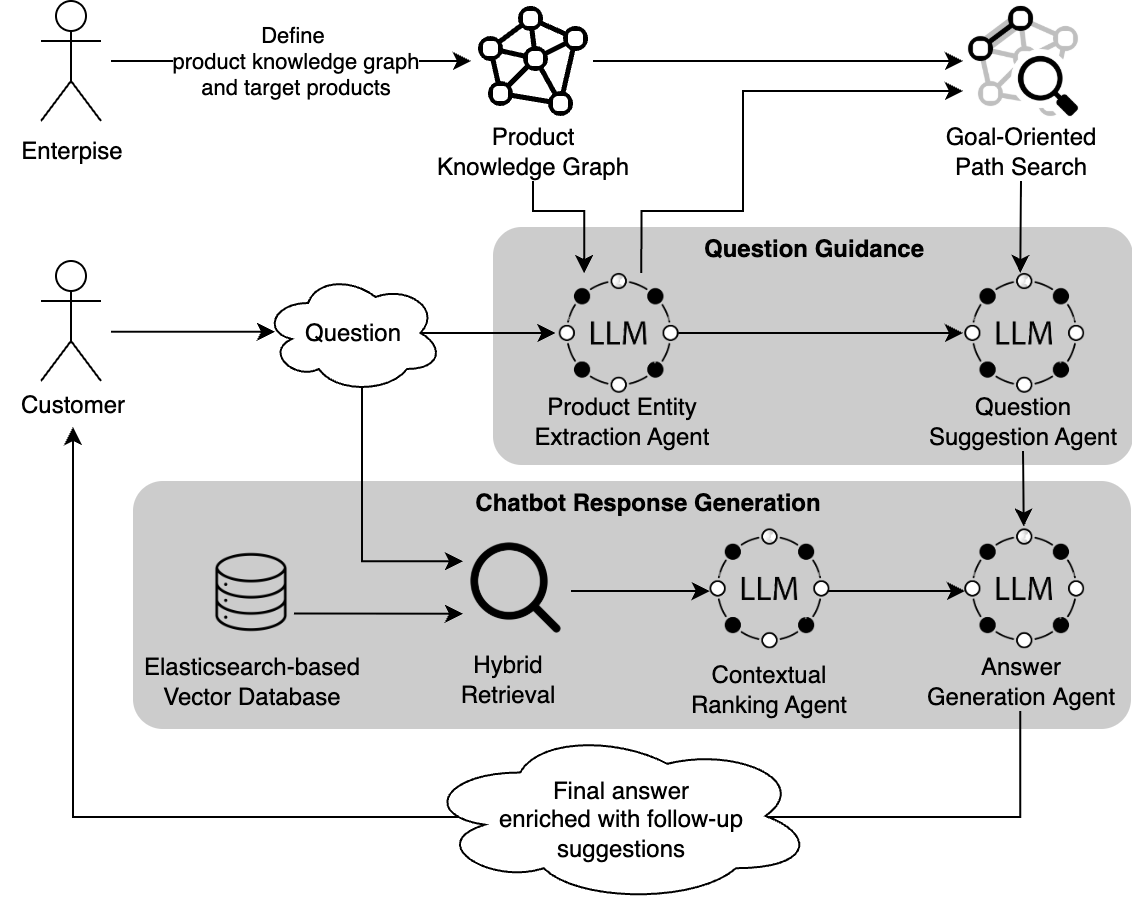
\includegraphics[width=0.5\textwidth]{Figure/overall_flow.png}}
    \caption{The overall architecture of the multi-agent chatbot with goal-oriented question suggestion.}
    \label{fig:architecture}
\end{figure}


\subsection{Question Guidance Component}

This component is responsible for generating suggestion questions to guide the conversation toward business-defined goals. It consists of two LLM-based agents: the \textit{Product Entity Extraction Agent} and the \textit{Question Suggestion Agent}.


% \subsection{Thành phần Gợi ý}
% Thành phần này chịu trách nhiệm tạo ra các câu hỏi gợi ý để dẫn dắt cuộc hội thoại. Nó bao gồm Tác tử Nhận dạng Thực thể và Tác tử Gợi ý Tự nhiên.

\textbf{Product Entity Extraction Agent:} When the user poses a query, this agent identifies the names of smartphone products mentioned in the utterance. It uses a large language model prompted for the Named Entity Recognition (NER) task. The extracted product names are then matched against the product knowledge graph using fuzzy search techniques to locate the corresponding source nodes.

% \textbf{Tác tử Nhận dạng Thực thể (NER Agent):} Khi người dùng đặt câu hỏi, tác tử này có nhiệm vụ trích xuất tên của các sản phẩm smartphone được đề cập. Agent là một LLM với prompt được thiết kế cho tác vụ Named Entity Recognition (NER). Tên sản phẩm được trích xuất sau đó được đối chiếu với cơ sở dữ liệu bằng kỹ thuật tìm kiếm mờ (fuzzy search) để xác định chính xác nút thực thể nguồn trong đồ thị tri thức.

\textbf{Question Suggestion Agent:} This agent receives as input a set of high-scoring paths from the knowledge graph traversal algorithm. For each path, it extracts a triplet consisting of the source product, the next product along the path, and the semantic relationship connecting them. Based on this triplet, the agent generates two outputs: a \textit{rationale sentence} and a \textit{follow-up question}. 

The \textit{rationale sentence} provides a natural-language explanation of why the next product is relevant. For example: \textit{“Alongside the Samsung Galaxy S25, another phone in the same price range of 20–25 million VND that you might find interesting is the iPhone 15.”}

The \textit{follow-up question} is a targeted inquiry about the suggested product, designed to encourage further user engagement. For instance: \textit{“Would you like to explore how the iPhone 15’s performance compares to the previous model?”}

% \textbf{Tác tử Gợi ý Tự nhiên (Natural Recommendation Agent):} Tác tử này nhận đầu vào là các đường đi tối ưu từ thuật toán tìm kiếm trên đồ thị tri thức. Với mỗi đường đi, nó lấy ra bộ ba dữ liệu bao gồm: sản phẩm nguồn, sản phẩm ngay sau sản phẩm nguồn trên đường đi, và quan hệ giữa hai sản phẩm này. Dựa trên thông tin này, nó tạo ra một lời giải thích gợi ý và một câu hỏi gợi ý. \textbf{Lời giải thích} là một câu văn tự nhiên giải thích lý do tại sao sản phẩm tiếp theo lại liên quan. Ví dụ: \textit{"Bên cạnh chiếc Samsung Galaxy S25, một chiếc điện thoại khác trong cùng tầm giá 10-11 triệu mà bạn có thể quan tâm là iPhone 15."}
% \textbf{Câu hỏi gợi ý} là một câu hỏi cụ thể về sản phẩm được gợi ý, khuyến khích người dùng khám phá thêm. Ví dụ: \textit{"Bạn có muốn tìm hiểu về cấu hình của iPhone 15 có cải tiến gì so với phiên bản trước không?"}

On the chatbot interface, the \textit{rationale sentence} is appended directly to the previous system response, while the \textit{follow-up questions} are displayed below as clickable options for the user. This design enables a seamless connection between the suggested product (e.g., iPhone 15) and the user's current interest (e.g., Samsung Galaxy S25) as they share the same attribute value, such as price range. The follow-up questions, however, are not constrained to this specific attribute; they are designed to encourage broader exploration of the suggested product across multiple dimensions.

% Trên giao diện chatbot, câu giải thích sẽ nối luôn vào câu trả lời cho câu hỏi trước và ở dưới câu trả lời sẽ hiện các câu hỏi tiếp theo để người dùng bấm vào. Nhờ đó, sản phẩm mới (iPhone 15) được liên kết tự nhiên với sản phẩm trước (Samsung galaxy s25) bằng mức giá, nhưng các câu hỏi gợi ý đặt ra sẽ rộng hơn là mức giá và đặt về nhiều trường thông tin khác của sản phẩm mới.

The agent is implemented using a large language model with a few-shot prompting approach, where a small set of input-output examples is embedded in the prompt to guide the model toward generating the desired outputs.

% Tác tử này được triển khai bằng LLM với kỹ thuật few-shot prompting, nơi một vài ví dụ đầu vào-đầu ra mẫu được cung cấp trong prompt để định hướng cho LLM tạo ra kết quả mong muốn.

\subsection{Chatbot Response Generation Component}
\label{sec:chatbot_response}

This component is responsible for answering user questions, whether they are initiated directly by the user or selected from system-generated suggestions. The chatbot is implemented using a Retrieval-Augmented Generation (RAG) architecture, which allows it to dynamically combine language generation capabilities with knowledge retrieved from a product database.


% \subsection{Thành phần Chatbot}
% Thành phần này chịu trách nhiệm trả lời các câu hỏi của người dùng, dù đó là câu hỏi do người dùng chủ dộng tự đưa ra hay câu hỏi được chọn từ gợi ý của hệ thống. Chatbot này được  triển khai dựa trên kiến trúc truy xuất Tăng cường (Retrieval-Augmented Generation - RAG) như sau.

To construct the knowledge base, we collected all textual content related to smartphone products from the Vietnamese e-commerce website \textit{Thegioididong.com}. The data was processed and segmented into meaningful chunks while preserving the structural integrity of the source, such as avoiding splits between section headers and their corresponding content. These text segments were then embedded into dense vector representations using Google's \texttt{text-embedding-004} model and stored in an Elasticsearch-based vector database.


% Để \textbf{xây dựng cơ sở tri thức}, toàn bộ nội dung văn bản liên quan đến sản phẩm smartphone được thu thập từ trang thương mại điện tử Thegioididong.com. Dữ liệu này được xử lý và phân mảnh (chunking) một cách thông minh, tôn trọng cấu trúc của trang web (ví dụ, không cắt ngang giữa một tiêu đề và nội dung của nó). Các mảnh văn bản này sau đó được mã hóa thành các vector nhúng (embedding) bằng mô hình \texttt{text-embedding-004} của Google và được lưu trữ trong cơ sở dữ liệu vector Elasticsearch.

When a user submits a query, the RAG pipeline is triggered with a \textit{hybrid retrieval} mechanism. Instead of relying solely on vector-based semantic search, we adopt Elasticsearch’s Reciprocal Rank Fusion (RRF) hybrid search strategy, which combines results from both traditional lexical search (BM25) and dense vector search. This approach leverages the strengths of both methods: BM25 excels at retrieving exact keyword matches such as model names or technical specifications, while vector search offers superior performance in capturing user intent and semantic relevance.

% Khi có một câu hỏi từ người dùng, luồng xử lý RAG diễn ra với cơ chế \textbf{Tìm kiếm Hybrid}. Thay vì chỉ dựa vào tìm kiếm vector (tìm kiếm ngữ nghĩa), chúng tôi sử dụng cơ chế Reciprocal Rank Fusion (RRF) Hybrid Search của Elasticsearch. Cơ chế này kết hợp kết quả từ cả tìm kiếm từ khóa truyền thống (BM25 - lexical search) và tìm kiếm vector (dense vector search). Sự kết hợp này tận dụng thế mạnh của cả hai phương pháp: BM25 xuất sắc trong việc tìm các từ khóa chính xác như tên model, thông số kỹ thuật, trong khi tìm kiếm vector lại vượt trội trong việc hiểu ý định và ngữ nghĩa của người dùng.

The retrieved text chunks are passed to an LLM-based \textit{Contextual Ranking Agent}, which filters out irrelevant segments and reorders the remaining ones based on their semantic relevance to the user query. The top-ranked segments are then provided as contextual input to the \textit{Answer Generation Agent}, which synthesizes the information and generates a complete, coherent response in Vietnamese.

% Các mảnh văn bản được truy xuất từ bước tìm kiếm sẽ được đưa vào tác tử LLM-based \textbf{Tái xếp hạng (Rerank Agent)}. Tác tử này có nhiệm vụ lọc bỏ các mảnh không liên quan và xếp hạng lại những mảnh còn lại dựa trên mức độ phù hợp với câu hỏi. Cuối cùng, các mảnh văn bản đã được lọc và xếp hạng sẽ được cung cấp làm ngữ cảnh cho tác tử \textbf{Trả lời (Answer Agent)}. Tác tử này tổng hợp thông tin và tạo ra một câu trả lời hoàn chỉnh, tự nhiên bằng tiếng Việt.




% Sự tích hợp giữa Thành phần Gợi ý và Thành phần Chatbot cho phép tạo ra một luồng hội thoại liền mạch. Câu trả lời của chatbot không chỉ giải đáp thắc mắc mà còn mở đường cho các gợi ý từ thành phần gợi ý, tạo ra một vòng lặp tương tác chủ động và thông minh.

\section{User Simulation for System Evaluation}\label{sec:user_simulation}

One of the main challenges in developing conversational systems is the evaluation process. Testing with real users is expensive, time-consuming, and difficult to control due to numerous external variables. Moreover, unless participants are genuinely interested in purchasing a product, their responses may be biased or inconsistent, which undermines the objectivity of the evaluation. To address these challenges, we developed a simulated environment in which an LLM-based \textit{Simulated User Agent} plays the role of a human user and interacts with the chatbot system.


% \section{User Behaviour Simulation}
% Một trong những thách thức lớn nhất khi phát triển các hệ thống hội thoại là việc đánh giá hiệu quả. Việc thử nghiệm với người dùng thật tốn kém, mất thời gian và khó kiểm soát các biến số. Để khắc phục điều này, chúng tôi đã xây dựng một môi trường mô phỏng, trong đó một \textbf{Tác tử Người dùng (User Agent)} dựa trên LLM sẽ đóng vai người dùng để tương tác với chatbot.


\subsection{Simulated User Modeling for Interaction Testing}

To realistically simulate user behavior, the \textit{Simulated User Agent} makes decisions based on two primary inputs: (i) a fixed \textbf{User Profile} and (ii) the evolving \textbf{Dialogue Context}.

% \subsection{Thiết kế Tác tử Người dùng}
% Để mô phỏng hành vi của người dùng một cách thực tế, Tác tử Người dùng sử dụng hai thông tin đầu vào là (i) hồ sơ cá nhân và (ii) ngữ cảnh hội thoại để ra quyết định.

The \textbf{User Profile} remains constant throughout a session and comprises two key components: a \textit{user persona} and a \textit{synthetic interaction history}. The persona defines the user's behavioral archetype, such as a student, business professional, elderly user, or mobile gamer. Each persona is specified with detailed characteristics, shopping motivations, and decision patterns. For instance, a student persona is defined by a limited budget and high sensitivity to promotions.

The interaction history simulates prior purchases and inquiries, providing the agent with an initial set of interests before the conversation begins. This profile-driven structure supports more realistic and context-aware behavior as the dialogue unfolds.


% \textbf{Hồ sơ người dùng (User Profile)} được giữ cố định trong suốt một phiên hội thoại; nó bao gồm \textit{đặc điểm nhân vật} và \textit{lịch sử tương tác}. Để xây dựng \textit{đặc điểm nhân vật}, tác tử được chỉ định ngẫu nhiên để đóng một trong 10 vai trò người dùng khác nhau (ví dụ: Học sinh, Doanh nhân, Người lớn tuổi, Game thủ). Mỗi vai trò đi kèm với một mô tả chi tiết về đặc điểm, nhu cầu, và hành vi mua sắm. Ví dụ, một "Học sinh" sẽ có ngân sách hạn hẹp và quan tâm đến các chương trình khuyến mãi. Để xây dựng \textit{Lịch sử tương tác}, một lịch sử giả lập về các sản phẩm đã mua và đã hỏi trước đó được tạo ngẫu nhiên. Điều này giúp Tác tử Người dùng hình thành các mối quan tâm ban đầu trước khi bắt đầu cuộc trò chuyện.

The \textbf{Dialogue Context} captures the full conversation history, including the user's previous questions, the chatbot’s responses, and any suggested follow-up questions. The agent is instructed to prioritize the most recent question–answer exchanges in order to make context-aware decisions for the next turn.


% \textbf{Ngữ cảnh hội thoại (Conversation Context)} là toàn bộ lịch sử trò chuyện của người dùng, bao gồm câu hỏi trước đó, câu trả lời của chatbot và các gợi ý mới. Nó được yêu cầu tập trung vào những thông tin gần nhất để đưa ra quyết định tiếp theo.

Based on the User Profile and Dialogue Context, the Simulated User Agent selects one of two actions: \textbf{Accept}, by choosing a suggested follow-up question; or \textbf{Reject}, by ignoring all suggestions and generating a new question based on the character’s internal thoughts and needs.

To promote behavioral diversity and unpredictability, we set a high \texttt{temperature} value for the language model, enabling the agent to act in a more human-like and non-deterministic manner.


% Dựa trên hồ sơ người dùng và ngữ cảnh hội thoại, Tác tử Người dùng sẽ đưa ra một trong hai quyết định: \textbf{Chấp nhận (Accept)} -- Chọn một trong các câu hỏi được hệ thống gợi ý, hoặc (ii) \textbf{Từ chối (Reject)} -- Bỏ qua tất cả các gợi ý và tự tạo ra một câu hỏi mới dựa trên "suy nghĩ" và "nhu cầu" của nhân vật mà nó đang đóng vai.
% Chúng tôi thiết lập tham số \texttt{temperature} (mức độ sáng tạo) của LLM ở mức cao, giúp đảm bảo hành vi của Tác tử Người dùng có tính ngẫu nhiên và khó đoán, mô phỏng gần hơn với người dùng thật.

\subsection{User Simulation Flow and Termination Criteria}

A simulation session is a multi-turn conversation between the Simulated User Agent and the chatbot system. %The full interaction flow is illustrated in Figure~\ref{fig:simulation}. 
A session is labeled as a \textbf{success} if the user eventually asks about the target product. It is marked as a \textbf{failure} under either of the following conditions: (i) the number of dialogue turns exceeds a preset threshold (e.g., six turns) without reaching the target, or (ii) the Simulated User Agent rejects suggestions leading to the target product more than twice.

All user utterances, agent decisions, and intermediate system outputs are logged to support detailed analysis and system evaluation.

% \subsection{Luồng Mô phỏng và Điều kiện Dừng}
% Một phiên mô phỏng là một cuộc hội thoại nhiều lượt giữa Tác tử Người dùng và hệ thống chatbot. Luồng mô phỏng được thể hiện trong Hình \ref{fig:simulation}.
% Mỗi phiên mô phỏng sẽ kết thúc \textbf{Thành công (Success)} khi Tác tử Người dùng đặt một câu hỏi về sản phẩm mục tiêu, hoặc sẽ được xác định là \textbf{Thất bại (Fail)} khi hoặc (i) cuộc hội thoại vượt quá một số lượt nhất định (ví dụ, 6 lượt) mà vẫn chưa đạt được mục tiêu, hoặc (ii) tác tử Người dùng từ chối các gợi ý dẫn đến sản phẩm mục tiêu quá 2 lần.


% Toàn bộ cuộc hội thoại, các quyết định của Tác tử Người dùng, và các thông tin trung gian đều được ghi lại để phục vụ cho việc phân tích và lượng giá hiệu quả của hệ thống.

% \begin{figure*}[!t]
%     \centerline{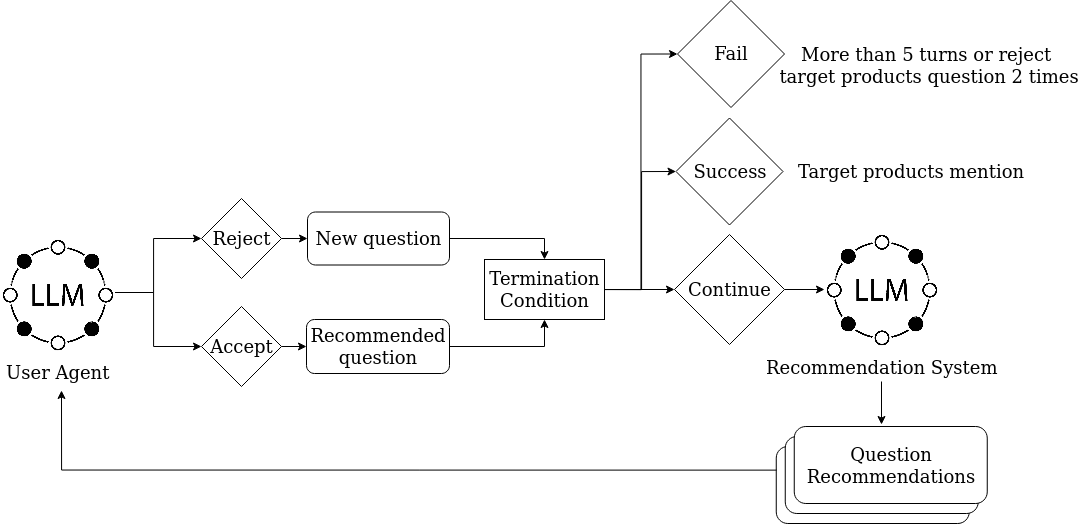
\includegraphics[width=\textwidth]{Figure/simulation_flow.png}}
%     \caption{Interaction flow of the User Simulation, detailing the Conversation Loop and Termination Conditions.}
%     \label{fig:simulation}
% \end{figure*}

\section{Experimental Setup, Results, and Evaluation}\label{sec:evaluation}

To assess the effectiveness of the proposed system, we conducted a series of 20 simulation sessions, each representing a distinct synthetic user with a unique persona and product goal. The goal of these experiments is twofold: (i) to verify whether the system can successfully guide users toward target products in natural conversations, and (ii) to evaluate the contribution of each core component. To this end, we designed two ablation scenarios: the first disables the personalized user interaction history, and the second removes the product knowledge graph, thereby eliminating structured path guidance. These comparisons provide insight into the impact of personalization and graph-based reasoning on the overall system performance.

We acknowledge that our evaluation is limited to 20 simulated sessions and lacks validation with real-world users. Although the LLM-based simulation provides a cost-efficient and repeatable approach, it cannot fully capture the complexity of human behavior. In addition, we did not compare against proactive recommendation baselines such as Iterative Preference Guidance (IPG) \cite{bi2024proactive} or multivariate policy learning \cite{jeunen2024multi}. Direct comparison remains difficult because most baselines are designed for offline recommendation or static datasets, whereas our system operates in a dynamic conversational environment that combines multi-turn dialogue with knowledge graph reasoning. Incorporating adapted baselines into future work will help establish a stronger empirical foundation for our contributions.

% We acknowledge that our evaluation is limited to 20 simulated sessions, without validation on real-world user interactions. While the LLM-based simulation offers a cost-efficient and repeatable method, it cannot fully substitute for actual human behavior. Furthermore, we have not compared against existing proactive recommendation baselines such as Iterative Preference Guidance (IPG) \cite{bi2024proactive} or multivariate policy learning \cite{jeunen2024multi}. A direct comparison is challenging because most baseline methods are designed for offline recommendation or static datasets, whereas our system operates in a dynamic conversational environment that integrates multi-turn dialogue and knowledge graph reasoning. Nevertheless, incorporating adapted baselines in future work will provide a stronger empirical position for our contributions.



% Nghiên cứu đã tiến hành thực nghiệm bằng cách chạy 20 phiên mô phỏng, tương ứng với 20 người dùng giả lập có hồ sơ và sản phẩm mục tiêu khác nhau. Để đánh giá vai trò của từng thành phần cốt lõi, chúng tôi thực hiện phương pháp đánh giá theo từng phần (component-wise evaluation) với hai kịch bản chính.

\subsection{Evaluation Metrics}

To evaluate the system's performance from both user-centric and business-driven perspectives, we define the following metrics:

\begin{itemize}
    \item \textbf{History Match Rate:}  
    % The proportion of recommendation turns where the suggested product matches an item from the user's past interactions.
    The proportion of turns in which the system’s suggested question contains a product that appears in the user's past interactions.
    This reflects the system's ability to tailor suggestions based on user history.
    
    \item \textbf{Acceptance Rate:}  
    The proportion of times the user accepts a system-suggested question. This measures user engagement and perceived relevance.
    
    \item \textbf{Answerability Rate:}  
    The proportion of suggested questions that the chatbot is able to answer, indicating the alignment between the Question Guidance Component and the chatbot's knowledge base.
    
    \item \textbf{Goal Completion Rate:}  
    The percentage of sessions that successfully end with the user inquiring about the target product. This is the primary metric reflecting business success.
\end{itemize}

% Để lượng giá sự hữu ích hệ thống theo cả hai hướng cho người dùng và doanh nghiệp, chúng tôi định nghĩa các chỉ số đánh giá như sau.
% \begin{itemize}
%     \item \textbf{P\textsubscript{user\_info} (Tỉ lệ gợi ý liên quan):} Tỉ lệ các lượt hội thoại có gợi ý chứa sản phẩm mà người dùng đã tương tác trong quá khứ. Chỉ số này đo lường mức độ cá nhân hóa.
%     \item \textbf{P\textsubscript{user\_acceptance} (Tỉ lệ chấp nhận gợi ý):} Tỉ lệ người dùng chấp nhận câu hỏi gợi ý của hệ thống.
%     \item \textbf{P\textsubscript{chatbot\_compatibility} (Tỉ lệ tương thích gợi ý):} Tỉ lệ các câu hỏi gợi ý mà chatbot có khả năng trả lời (nằm trong phạm vi tri thức của chatbot).
%     \item \textbf{P\textsubscript{target\_arrival} (Tỉ lệ đạt mục tiêu):} Tỉ lệ các phiên hội thoại kết thúc thành công (người dùng hỏi về sản phẩm mục tiêu). Đây là chỉ số quan trọng nhất để đo lường hiệu quả kinh doanh.
% \end{itemize}

% \subsection{Ablation on Personalization}
\subsection{Impact of Personalization}

% \subsection{Kịch bản 1: Lượng giá vai trò của Cá nhân hóa (User-oriented)}
% In this experiment, we assess the impact of personalization by comparing the full system with a variant that removes user history from the path scoring function. Results in Table~\ref{tab:result_user_oriented} show a dramatic drop in \textit{History Match Rate} from 79.6\% to 2.3\% without access to prior interactions. This indicates that the system becomes almost incapable of recommending products previously shown to interest the user. As a consequence, the \textit{Acceptance Rate} also declines. These results highlight the importance of incorporating user history to generate relevant suggestions and sustain user engagement.


In this scenario, we compare the full system with a variant that removes user interaction history from the path scoring function. Results in Table~\ref{tab:result_user_oriented} show that excluding personalization causes the \textbf{History Match Rate} to plummet from 79.6\% to just 2.3\%, indicating that the system becomes almost entirely unable to recommend products previously aligned with the user’s interests. This reduction also leads to a noticeable drop in the \textbf{Acceptance Rate}, confirming that user history plays a vital role in generating compelling suggestions and maintaining engagement.


% Trong kịch bản này, chúng tôi so sánh hệ thống hoàn chỉnh với một phiên bản hệ thống đã loại bỏ thông tin về lịch sử tương tác của người dùng (\texttt{H}) ra khỏi thuật toán chấm điểm đường đi. Kết quả được thể hiện trong Bảng \ref{tab:result_user_oriented} cho thấy khi loại bỏ thông tin cá nhân hóa, chỉ số \texttt{P\_user\_info} giảm mạnh từ 79.6\% xuống chỉ còn 2.3\%. Điều này chứng tỏ hệ thống gần như không thể gợi ý các sản phẩm mà người dùng đã từng quan tâm. Hệ quả là tỉ lệ chấp nhận gợi ý (\texttt{P\_user\_acceptance}) cũng giảm nhẹ. Điều này khẳng định tầm quan trọng của việc tích hợp lịch sử người dùng để tạo ra các gợi ý hấp dẫn và duy trì sự tương tác.

\begin{table}[!t]
    \centering
    \caption{Comparison with and without user history information.}
    \label{tab:result_user_oriented}

    \begin{tabularx}{\columnwidth}{@{} l 
        >{\centering\arraybackslash}X 
        >{\centering\arraybackslash}X 
        >{\centering\arraybackslash}X 
        >{\centering\arraybackslash}X @{}}
        \toprule
        \textbf{System} & 
        \textbf{HMR} & 
        \textbf{AR} &
        \textbf{ACR} & 
        \textbf{GCR} \\
        \midrule
        Full System & 79.6\% & 94.7\% & 52.0\% & 20.0\% \\
        No User History & 2.3\% & 94.4\% & 46.0\% & 20.0\% \\
        \bottomrule
    \end{tabularx}

    \vspace{2mm}
    \footnotesize
    \textbf{HMR}: History Match Rate \quad
    \textbf{AR}: Answerability Rate \\
    \textbf{AcR}: Acceptance Rate \quad
    \textbf{GCR}: Goal Completion Rate
\end{table}



% \begin{table}[!t]
%     \centering
%     \caption{So sánh hiệu năng khi có và không có thông tin lịch sử người dùng.}
%     \label{tab:result_user_oriented}

%     \begin{tabularx}{\columnwidth}{@{} l >{\centering\arraybackslash}X >{\centering\arraybackslash}X >{\centering\arraybackslash}X @{}}
%         \toprule
%         \textbf{Luồng hệ thống} & 
%         \textbf{$P_{\text{user\_info}}$} & 
%         \textbf{$P_{\text{user\_acceptance}}$} & 
%         \textbf{$P_{\text{target\_arrival}}$} \\
%         \midrule
%         Hệ thống hoàn chỉnh & 0.7963 & 0.52 & 0.2 \\
%         Loại bỏ Lịch sử người dùng & 0.0227 & 0.46 & 0.2 \\
%         \bottomrule
%     \end{tabularx}
% \end{table}




% \subsection{Kịch bản 2: Lượng giá vai trò của Đồ thị tri thức (Business-oriented)}
\subsection{Impact of Knowledge Graph on Business-Oriented Goals}

In this scenario, we remove the knowledge graph component entirely. Instead of guiding the conversation through intermediate entities, the Question Suggestion Agent attempts to create direct recommendations from the user's current query to the target product.

The results in Table~\ref{tab:result_business_oriented} show a substantial decline in system performance when the knowledge graph is removed. In particular, the \textbf{Goal Completion Rate} drops to zero, indicating that the system is unable to guide users to the target product. Without structural support, it lacks logical transitions between products, resulting in abrupt and unconvincing suggestions. For example, the system may suggest a high-end device immediately after the user inquires about a budget option, leading to repeated rejections from the Simulated User Agent.

Interestingly, the \textbf{History Match Rate} increases slightly in this scenario. This is likely because user history is still embedded in the prompt, which may lead the model to overfit to previously mentioned items. However, the improvement is minimal and does not compensate for overall decline in coherence and goal alignment caused by the lack of graph-based reasoning.

The absence of the graph also negatively impacts the \textbf{Answerability Rate}, as the model becomes more prone to hallucinating or producing off-topic suggestions when it is no longer grounded by structured relational context. These findings highlight the pivotal role of the product knowledge graph in generating coherent, goal-aligned recommendations that meet both user expectations and business objectives.


% Furthermore, the Answerability Rate also decreases, highlighting the tendency of the LLM to generate hallucinated or off-topic suggestions when not grounded by the graph. These findings confirm that the knowledge graph is a critical component for achieving coherent recommendations and supporting business objectives.


% Trong kịch bản này, chúng tôi loại bỏ hoàn toàn thành phần đồ thị tri thức. Thay vào đó, Tác tử Gợi ý sẽ cố gắng tạo gợi ý trực tiếp từ sản phẩm người dùng đang hỏi đến sản phẩm mục tiêu mà không có các bước trung gian. Kết quả được thể hiện trong Bảng \ref{tab:result_business_oriented} cho thấy một sự sụt giảm nghiêm trọng trên mọi phương diện. Đáng chú ý nhất, tỉ lệ đạt mục tiêu (\texttt{P\_target\_arrival}) giảm xuống 0\%. Điều này xảy ra vì khi không có đồ thị tri thức, hệ thống không thể tìm ra một con đường logic để kết nối sản phẩm. Các gợi ý trở nên đột ngột và thiếu tự nhiên (ví dụ: đang hỏi về một sản phẩm giá rẻ, lại được gợi ý ngay một sản phẩm cao cấp), dẫn đến việc Tác tử Người dùng liên tục từ chối. Hơn nữa, \texttt{P\_chatbot\_compatibility} cũng giảm, cho thấy LLM có xu hướng "ảo giác" và tạo ra các gợi ý nằm ngoài phạm vi tri thức của chatbot khi không có sự ràng buộc từ đồ thị. Kết quả này chứng minh rằng đồ thị tri thức là thành phần tối quan trọng để đạt được mục tiêu kinh doanh.


\begin{table}[!t]
    \centering
    \caption{Performance comparison with and without the knowledge graph}
    \label{tab:result_business_oriented}
    \begin{tabularx}{\columnwidth}{@{} l 
        >{\centering\arraybackslash}X 
        >{\centering\arraybackslash}X 
        >{\centering\arraybackslash}X 
        >{\centering\arraybackslash}X @{}}
        \toprule
        \textbf{System Variant} & 
        \textbf{HMR} & 
        \textbf{AR} & 
        \textbf{AcR} & 
        \textbf{GCR} \\
        \midrule
        Full System & 79.6\% & 94.7\% & 52.0\% & 20.0\% \\
        Without Knowledge Graph & 81.2\% & 63.3\% & 40.0\% & 0.0\% \\
        \bottomrule
    \end{tabularx}

    \vspace{2mm}
    \footnotesize
    \textbf{HMR}: History Match Rate \quad
    \textbf{AR}: Answerability Rate \\
    \textbf{AcR}: Acceptance Rate \quad
    \textbf{GCR}: Goal Completion Rate
\end{table}


% \begin{table}[!t]
%     \centering
%     \caption{Performance comparison with and without knowledge graph}
%     \label{tab:result_business_oriented}

%     \begin{tabularx}{\columnwidth}{@{} l >{\centering\arraybackslash}X >{\centering\arraybackslash}X >{\centering\arraybackslash}X >{\centering\arraybackslash}X @{}}
%         \toprule
%         \textbf{\shortstack{System\\Variant}} & 
%         \textbf{\shortstack{History\\Match\\Rate}} & 
%         \textbf{\shortstack{Answer-\\ability\\Rate}} &
%         \textbf{\shortstack{Accepta-\\nce Rate}} & 
%         \textbf{\shortstack{Goal\\Completi-\\on Rate}} \\
%         \midrule
%         Full System & 79.6\% & 94.7\% & 52.0\% & 20.0\% \\
%         Without Knowledge Graph & 81.2\% & 63.3\% & 40.0\% & 0.0\% \\
%         \bottomrule
%     \end{tabularx}
% \end{table}




\section{Conclusion and Future Work}\label{sec:conclusion} 

This paper introduced a comprehensive and practical architecture for an e-commerce chatbot that integrates goal-oriented question recommendation. By combining a product knowledge graph, a multi-agent system powered by large language models, and a user simulation environment for evaluation, the proposed framework addresses the challenge of balancing user engagement with business-driven objectives.

Experimental results validate the critical roles of both personalization and structured guidance. Incorporating user history significantly increases the relevance and acceptance of suggested questions, while the knowledge graph provides the logical scaffolding needed to guide conversations coherently and drive users toward target products.

Future directions include automating knowledge graph construction and maintenance, enabling cross-category recommendation, and incorporating real-time personalization techniques to further enhance the system’s adaptability and effectiveness.


% \section{Conclusion}
% Bài báo này đã trình bày thành công một kiến trúc toàn diện và khả thi cho chatbot thương mại điện tử tích hợp hệ thống gợi ý câu hỏi định hướng mục tiêu. Bằng cách kết hợp một đồ thị tri thức sản phẩm, một hệ thống đa tác tử dựa trên LLM, và một môi trường mô phỏng để đánh giá, nghiên cứu đã giải quyết được bài toán cân bằng giữa việc phục vụ người dùng và việc thực hiện mục tiêu kinh doanh.

% Kết quả thực nghiệm đã khẳng định vai trò không thể thiếu của cả hai thành phần cốt lõi: (1) Việc tích hợp lịch sử người dùng giúp tăng đáng kể sự hấp dẫn và tỉ lệ chấp nhận của các gợi ý. (2) Đồ thị tri thức là xương sống cho phép hệ thống dẫn dắt cuộc hội thoại một cách logic và tự nhiên, và là yếu tố quyết định để đạt được các mục tiêu kinh doanh đã định trước.

% Hướng phát triển trong tương lai sẽ tập trung vào việc tự động hóa quá trình xây dựng và cập nhật đồ thị tri thức, mở rộng khả năng gợi ý liên danh mục (cross-category), và tích hợp các phương pháp cá nhân hóa thời gian thực (real-time personalization) để làm cho hệ thống ngày càng thông minh và hiệu quả hơn.

% \section*{References}

% Please number citations consecutively within brackets \cite{b1}. The 
% sentence punctuation follows the bracket \cite{b2}. Refer simply to the reference 
% number, as in \cite{b3}---do not use ``Ref. \cite{b3}'' or ``reference \cite{b3}'' except at 
% the beginning of a sentence: ``Reference \cite{b3} was the first $\ldots$''

% Number footnotes separately in superscripts. Place the actual footnote at 
% the bottom of the column in which it was cited. Do not put footnotes in the 
% abstract or reference list. Use letters for table footnotes.

% Unless there are six authors or more give all authors' names; do not use 
% ``et al.''. Papers that have not been published, even if they have been 
% submitted for publication, should be cited as ``unpublished'' \cite{b4}. Papers 
% that have been accepted for publication should be cited as ``in press'' \cite{b5}. 
% Capitalize only the first word in a paper title, except for proper nouns and 
% element symbols.

% For papers published in translation journals, please give the English 
% citation first, followed by the original foreign-language citation \cite{b6}.

\bibliographystyle{IEEEtranN}
\bibliography{references}

\end{document}
